\documentclass{article}
\usepackage[utf8]{inputenc}

\title{Lecture 3: Hypothesis testing }
\author{wbg231 }
\date{November 2022}
\usepackage{tikz,graphicx,amsmath,amsfonts,amscd,amssymb,bm,cite,epsfig,epsf,url}
\begin{document}
\maketitle
\begin{itemize}
\section{Finishing up last lecture }
\subsection{Moments}
    \item moment generally involves times, but this deals with movement around aspect of rotations, in terms of physics
    \item this is related to a motive in physics
    \item a moment is the turning force around a pivot
    \item the location of a fulcrum that balances a moment, is the mean of a weight distribution
    \item moments charicerize the shape of a probability distribution 
    \itme we are looking for the distrobution of the probaility mass   \item 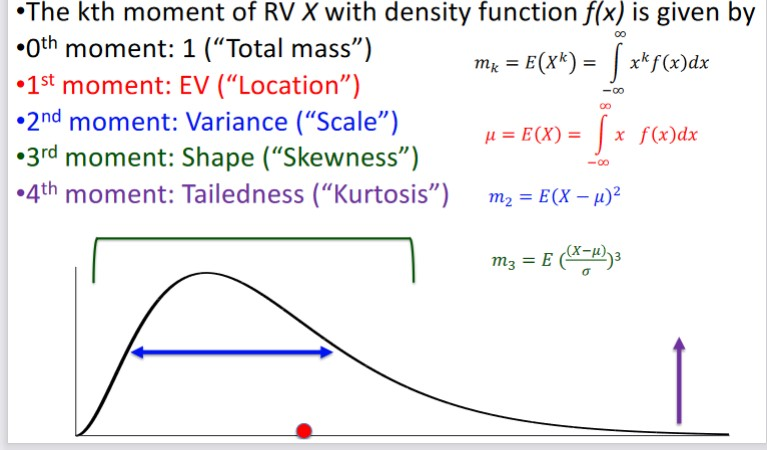
\includegraphics[width=10cm]{Final_Review/lecture_3/lecture 2 example 1 .jpg}

    \item so there is a center that ballances the forces
    \itme the kth moment a rv x with pdf $f(x)$ is $m_k=E(X^K)=\int x^kf(x)dx$
    \item the zeroth moment is $M_0=\int x^0f(x)dx=\int f(x)dx=1$ (think of this as total mass 
    \item so for k=1 $m_1=E(x^1)=\int x^1f(x)dx=E[x]$
    think of this as location in the sense that if you think of the pdf in real life and put it on a pivot the expected value is where it would balance. that is the red ball   
    \item k=2 we can write $m_2=E[X^2]=\int x^2f(x)dx$ this is variance it is a scale parameter it describes how spread out arround the mean the distorubiton is. this is teh blue line 
    .\item  the third moment is skewness it is how skewed the distrubiton 
    \item the 4th momenet is how heavy the distrobution is in effect.
    \subsection{Normal dist }
    \item one of the nicest moments we have 
    \item it is fully chacterized as by $\mu$, $\sigma$ the mean and variance 
    \item it is well behaved extreme events are unlikly 
    \item if we are in buisness and we think stuff is normaly distributed we can make good bets. 
    \item 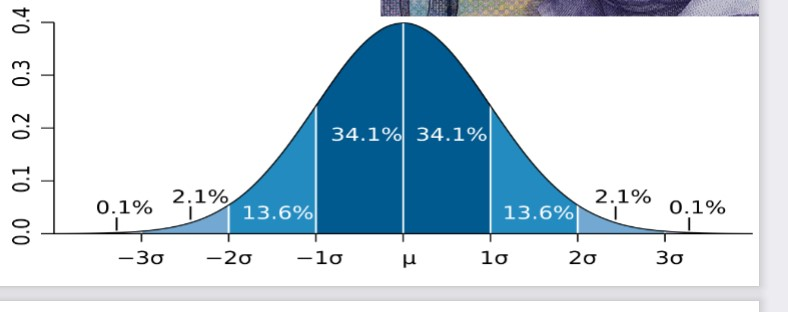
\includegraphics[width=10cm]{Final_Review/lecture_3/unfirom .jpg}
    \item everything is well described by the first two moments, but stuff is not always this nice 
    \item how do normal distrobutions come about? 
    \item the idea is if we drop balls at all the same time down a beg board it will reach a nroaml distribution 
    \item conditons for a normal dist
    \begin{enumerate}
        \item need many bernuli rv's
        \item need them to be inpatient 
    \end{enumerate}
    \item at each peg drop there are two paths each time. then it ends up with a pascalls triangle type shape. 
    \item pascalls triangle descirbes the number of paths of the balls following through each peg. 
    \item this is very satisfyinhg 
    \itme so in rela life a nroaml means that it si a physcical realization of these indpenint paths 
\subsection{Cauchy Distrobution }
\item both the expected vlaue adn vairnace are undefined 
high moments also unefeid
\item 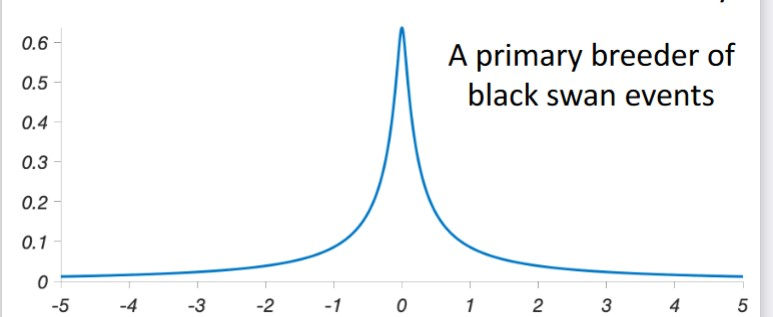
\includegraphics[width=10cm]{Final_Review/lecture_3/cauchy.jpg} 
\item the higher moments can sometimes be used 
\item extreme events are not that unlikely because the tails never relly reach 0. 
\item think iof the x axis as number of standard deviations from the mean
\itme in a normal distribution at 5 or -5 $\simga$ the chance of that occurring is basically 0, in a Cauchy distro that is not really the case, there is still some probaility density there 
\item so for instance if things are cauchy and you bet that something like -5, will never happen then you could lose a lot of your cash. if there are normally distrobutions these events will never happen. 
\item Cauchy distros are not that common, but they exist. and undermine our self 
\item in cauchy extreme events are unlikely but not vanishingly unluckily
\item so look the tials drop off genetly. 
\subsection{how does cauchy come about}
\item 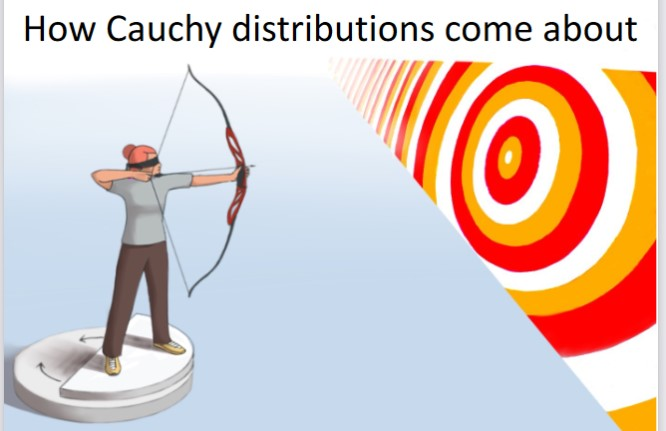
\includegraphics[width=10cm]{Final_Review/lecture_3/cauchy_archer.jpg} 
\item suppose there is an archer on a platofrm that rotates form 90 to -90 degrees, shooting arrows randomly at a wall of infinite legnth. we are assumign that there is no gravity, and that the guy shoots the arrow randomly.  
\item many of the archers arrows may hit the center of the distribution, but if they left go of the arrow at -89.999999 then the arroow can go very far off to the left side. 
\item so in the long term now expected value emerges
\item another example of a Cauchy could be the peg board, but if the events are not independent. 
\item so for instance getting a good job, getting the first one makes you mroe likely to get the second one and so on  
\item black swan events are when we have strong expecaions of things not happening but then they happen 
\item it is only a black swan if it is completly unexpceeted 
\section{Hypothesis testing material}
\subsection{Hypothsis testing introuduction }
\item we want to have a frame work to rationally aproach problems. 
\item this is at the heart of the scientific enterprise
\item this is not a proof it is a conclusion. 
\item hypothesis testing is science
\itme we are testing hypothesises 
\item science is rare in history 
\subsection{ the importance of hypothsis testing}
\item in europe in 15000 50,000 poeple were burned for witch craft 
\item witches do not exist
\item how did we do this so wrong? 
\item there was a guy who wrote a book about witches, there was a lot of social strife, then there was a witch trail that starts with a conclusion then looks for evidence to support that conclusion.  
\item confirmation bias, is when you are looking for facts to support your conclusions. 
\item blood letting was a main idea in medince for a long time 
\itme that basically came from Hippocrates
\item it took until the late 1800's for people to realize it was almost always a bad idea 
\item how could this go on for so long and no one notice? 
\item basically confirmation bais 
\item people look for evidence of what they already think.
\item bassically the human mind wants you to act as quikcly as possible, so it from a nueroogialc perspeictve makes sense to make a choice and work form that.
\item so there are evolutionary reaons to have conformaiton bias
\item science is a way to check conformation bias 
\subsection{thinking in terms of falsification}
\item  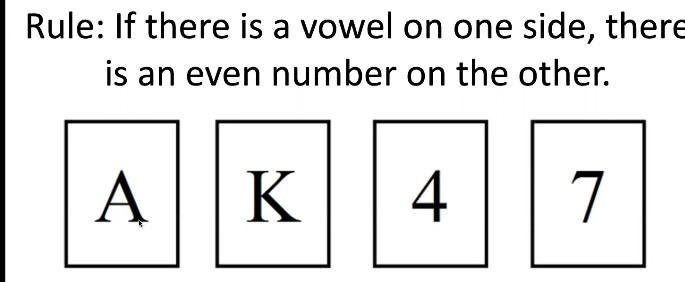
\includegraphics[width=5cm]{Final_Review/lecture_3/lecture 3 exmaple 2 .jpg} 
\item which cards do you have to turn over to test the rule? 

\item the A card of course, and then the 7 card.
\item first the a becuase if there is not an even number then the rule is violated 
\item we dont need the k becuase we know nothing about constants 
\item we dont need the 4 becuase the rule does not say that having an even on one side means there will be a vowel on the other
\item the 7 we do need to check becuase the rule says if there is a vowel on one side there must be an even on the other, so if there is a vowel on the other side of the 7 card this rule fails
\item example 2: if one is indoors one has to wear a mask. 
\begin{enumerate}
    \item person 1 is indoors: so if tehy are wearing a mask they are following the rule 
    \item person 2 is outdoors. this perosn we dont care about
    \item peron 3 is wearing a mask. this perosn we dont care about
    \item perosn 4 does not wear a mask. if they are indoors then they break the rule 
\end{enumerate}
\item it is hard to do this 
\item so we have made the null hypothsis signfigance testing to do this 
\itme is it counter intuitive so lets build up to it 
\subsection{sampleing }
\item out goal is to learn if something is true 
\item lets say that there is some fixed parameter $\theta$ in a population that is unknown
\item we will never get to see the full population os $\theta$ will alwyas be unknown 
\item so we need to esimate theta from a sample 
\item a sample is a subset of the populationt that we can measure 
\item we need to charter this sample in terms of a sample static statistics
\item so we hope that as the size of our sample goes to some large n we hope that our sample $\theta$ will approximate that of the population 
\item by sampleing with certian asumptions we can assume that the sample is simialr to the popoulation 
\subsection{example}
\item you are an epidemiology and you want to know the prevalence fo some disease in a village
\item assume that the true population parameter $\theta=.2$
\item if we take difrent sampels from the population we will have difrent estiamtes of $\theta$
\item as the size of those sampels goes up our esimate gets closer to the truth 
\item we can get a reasonably good esiamte with out samplign everyone 

\item  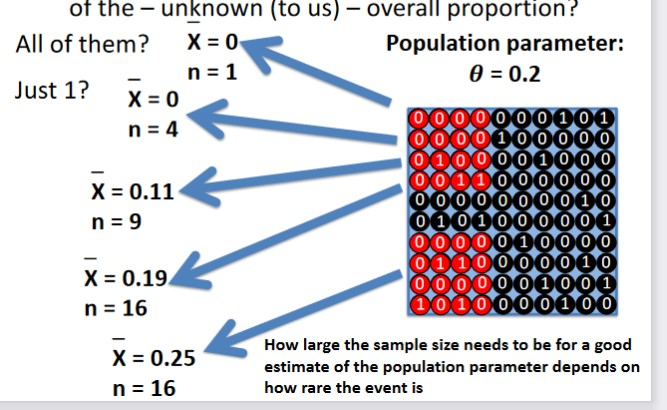
\includegraphics[width=5cm]{Final_Review/lecture_3/lecture 3 exmaple 23.jpg} 
\end{itemize}
\subsection{weak law of large numbers }
\item if teh sampleing from some rv x is indpendint and represnetative (IID meaning that each member of the popualtion as an equal chance of being in the sample) hten the sample eman will conver to the population mean as the sample size increases 
\item in other words let n be the popuation size $\epsilon$ be some arbitary small value and $\Bar{x}_n$ be our sample mean and $\mu$ be our populaiton mean  we have lim$_{n\rightarrow \infty}P(|\Bar{x_n}-\mu|\geq \epsilon)=0$
\item the iid assumption is required
\subsection{Central limit}
\item in short this says that if sampling randomly and independently then the sample means distribute normally as the same size increases regardless of how the underlying population is distributed. 
\item the sample means are a random variable 
\item this is the basis of statistics
\item it lets us quantify sampling error 

\item the sample size is the number of individuals in the sample
\item Suppose that we draw repeated random samples from teh same population t times. for each sample size n where n is the sample size of each sample. 
\item we then take the same mean $\Bar{x_t}$ for each sample $t_i$ and plot the distrobution of these tychenic sample means (this is more or less just saying that we are thinking of the sample mean as a random vairble that we are sampling from many times and then plotting it's distrobution) 
\item suppose we are looking to esiamte the number of times the average person in our population watches a netflix show
\item $\mu_{x}, \sigma_{x}$ are population mean and variance 
\itme $\Bar{X_i}, S_i$ are our tyrannic sample mean and standard deviations. that we use to estimate $\mu_x, \simga_x$ 
\item tychenic sample means, (not the data) form a distribution. and the mean of that distribution of our tychanci sample means is our esimtate of the populaiton mean 
\item and the width IE the standard deviation of the tychanic sample means, is out standard error of the sample mean (SEM) 
\item  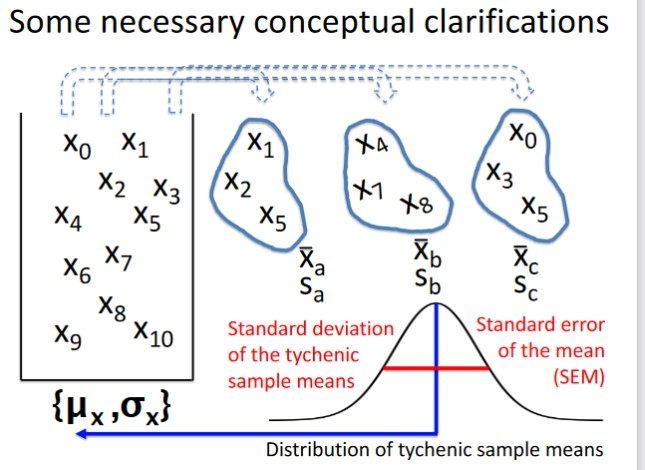
\includegraphics[width=5cm]{Final_Review/lecture_3/sample_mean_primer.jpg} 
\item the SEM is the standard deviation of the distribution of the sample means and is in the denominator of teh majority of hyptoshiss tests. 
\item recall that t the number of times we are resampling and n is teh number of samples. 
\item if we take n=1, t=10000 then we have many samples of size 1 from some population. if chosince each indivuda in that population is radnom then the distribution of the tycncanic sample means reflect the inital distorbution in this case normal 

\item  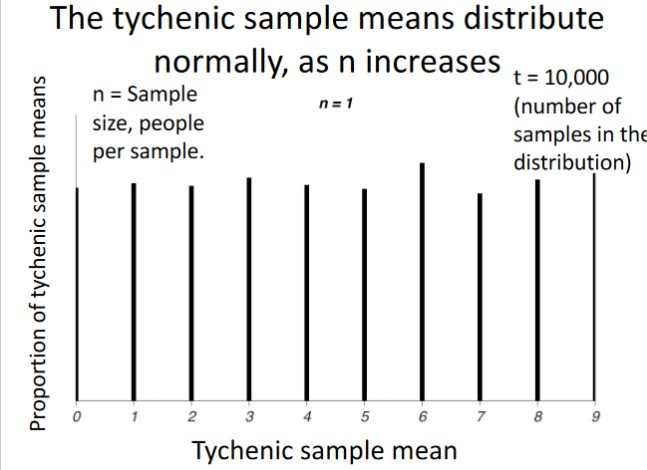
\includegraphics[width=5cm]{Final_Review/lecture_3/n=1.jpg} 
\item but if we keep our t large and increase n we see that the distrobution of the sample means aproach normal 
\item  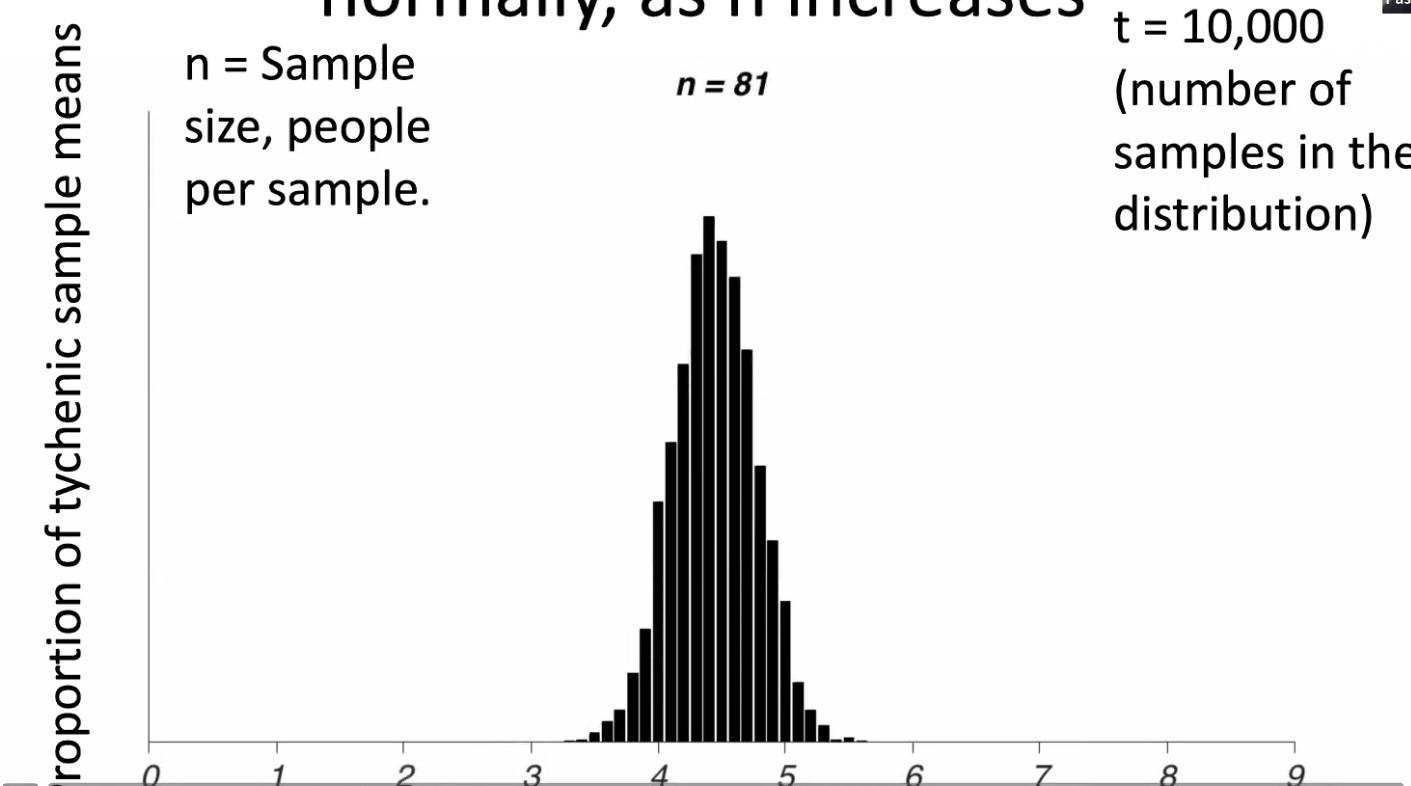
\includegraphics[width=5cm]{Final_Review/lecture_3/n=81.jpg}
\item it broadly becomes normal as n gets large
\item the larger the n the more normal meaning the more you can garuntee your ressutls. 
\item the standard deviation (standard error of the sample mean) of the sample means goes down as n goes up.
\item this works for any distrobution except for cauchy more or less
\item the reason this matters, is that if we get a large enough n we can garuntee some erorr bound for our sample mean. 
\subsection{what is the point}
\item in reality we can only do this once, that is get one sample of size n and can never know the true mean of the population 
\item but we want a reasonable chance that the sample eman of teh one sample you do have is a good enough estiamte of the unkown popualtion mena 
\item for this to happen we need to consider how scatterd/ varibles these sample means are 
\item We know that the standard error of the mean SEM does not drop linearlly as a function of sample size (n) instead SEM$=\sigma_{\Bar{x}}=\frac{\sigma}{\sqrt{n}}$ where $\simga$ is our true sample standard devation 
\item so we get diminishing returns to increasing our sample size. 
\subsection{where does SEM formula come from}
\item more or less what happens is the variance of our sample means goes down proportionally to the sample size that is $\simga_{\Bar{x}}^2=\frac{\sigma^2}{\sqrt{n}}$
\item but we are intrested in standard devation so we take the square root of both sides to get 
SEM$=\sigma_{\Bar{x}}=\frac{\sigma}{\sqrt{n}}$ where $\simga$ is our true sample standard deviation 
\item the larger the data set the larger sample size you need to get a certian SEM bound 
\subsection{CLT caveates}
\item The CLT reduces sampleing erorr sufficently if the sample is sufficently large
\item the meachnism behind this is that the larger the sample, the larger teh cahnce of random eror to cancel out effectifyly amplfying the singal 
\itme but this only works if we sample randomly 
\item if the sample is not taken randomly there are issues of sampling bias 
\item if there is sampleing bias then the sampleing error will not reduce as the CLT would sugest it would 
\subsection{example}
\item suppose there is a epedmic and we have a limited number of tests, but want to understnad how many poeple with the ilness die 
\item suppose we were to test the sickest people, maybe so we could care for them. so of the 10 poeple we test 10 have the dissease 1 dies then our case fitality rate is 10\%
\item if we tested the whole popoulation and only one person died the case fitality rate is just 1\%
\subsection{regression to the mean effect}
\item suppose that it has not rained for a really long time and then you do a rain dance and it starts to rain, did the rain dance make it rain? no, it had just not rained for longer than was normal so the chances of a conitnued streek of no rain went down 
\item another example, suppose there is a baseball team that is doing very unusually poorly for a long time then they fire the coach and the team starts to win more, is this casual? not nesscarilly they may have been for other reasons preforming in a way that was bellow the team's mean preofrmance (suppose we took a sample of 5 gaves all of which the team lost), they may just start doing better regardless of the coach becuase they were underprerforming not becuase the distrobution of team preformance has changed. 
\subsection{scinetific expirment}
\item in common language it means try something see what happens 
\item in math a repeatable rporudce with a well defined set of possible outcomes 
\item a scientific experiment has the following features 
\begin{enumerate}
    \item the unit of analysis are assigned to defiant codnitons (Treatments) that you control
    \item the treatmets are called the indepndint vairble (IV) and are assigned at random allwoing us to avoid confounders 
    \item this systematic invertion whiel controlling for all other factors by randomziation allows us to conduel cassality by ellimating all unknwn confounders
    \item in other word, a change in y the dependint vairble must be caseus by a change in x the independent vairble 
    \item this is teh best way to study causality
\end{enumerate}
\subsection{what makes experiment specail}
\item systamticaly varying (x) to create several experimetnal conditons 
\item randomizaton: ie randomly assinging unit sof analyisis to these contions each to recive a particual levle of x 
\item these consitute an intervention 
\iten then we measure y
\item then we compare data form difrent x 
\item then logic: given randomzaitn teh change in y must be causes by change  x.
\item this allows us to contorl for all other confounders
\subsection{ab test}
\item we want to know if amking a button larger makes poeple click on them more 
\item suppose we let users chose if they want a large or small button then measure click rates, and adopt that design for everyone. this is a bad design because people are self selecting there button size, so there might be some confounder getting in the way of this casual effect. 
\item we need to randomly assign people to treatments, so that we can control for confounders. 
\subsection{statitical sigfigance}
\item in common language not statsically sigfgnat means not a big deal 
\item in science statsically sigfgant menas taht the observed outcome is unlikly to occour asusming random chance. 
\item  it does nto mean the null hypothsis is false 
\item stastical sifgannt does not mean importat big large or real, it has nothing to do with a hpyothsis 
\item stastical sigfgence deos mean: an observed result is unlikle to be due to chance alone 
\item formally \textbf{statically sigfgant means} the probaility of the data assuming that the null hypothsis is ture is less than the chose sigfngence level
\item this is a statement about the liklyhood of the data
\item also it is probailistic so it does not prove anyhting 
\item we can be wrong 
\item so in science we are intrested in P(Data|null is True)
\item this is nice because all we need is the data. if we are doing bayes we need priors 
\item there is always a chance of sampling error. the real question is how likely is that due to chance. 
\subsection{Example}
\item suppose that the liklyhood of someone being smarter than the median is .5
\item we give a treatment to one person and they are smarter than the mean $P(x_1=1|t=1)=.5$ just by chance 
\item suppsoe we get a sample size of 2 peolpe, give them both the durg  and assume they are both smarter than average (assuming the treatment does not work and they are indepndient $P(X_1=1,x_2=1)=\frac{1}{4}$
\item so the likelihood of seing n poeple who are all brighter than avrage making tehse assumings is $P(\cap_{i=1}^{n}x_i=1)=\frac{1}{2^n}$
\item what is the threshold? most just use $\alpha=.05$
\item so that is we call something statiscally sigfgance if $P(X|null)\geq \alpha$
\subsection{significance levels}
\item denoted as $\alpha$
\item in princple we can use any levle we want the standard is $\alpha=.05$ that is $\frac{1}{20}$
\item this value just comes form fisher, he said it was good for compuation more or less. 
\end{document}
